% Clase 1 — Contexto, Historia IA y Agentes Inteligentes
% Lectura: AIMA Cap. 1-2
\section{Contexto e Historia de la IA}

\subsection{Impacto de la IA en el mundo real}

La IA impacta múltiples sectores: economía, política, ley y derecho, trabajo, ciencia, salud y educación.

\subsection{¿Qué es la Inteligencia Artificial?}

Existen cuatro enfoques para definir la IA:

\begin{center}
\begin{tabular}{|l|l|}
\hline
\textbf{Pensamiento humano} & \textbf{Pensamiento racional} \\
Modelos cognitivos & Leyes del pensamiento (lógica) \\
\hline
\textbf{Actuar humanamente} & \textbf{Actuar racionalmente} \\
Test de Turing & Agentes racionales \\
\hline
\end{tabular}
\end{center}

\begin{remark}
La IA moderna se enfoca en \textbf{agentes racionales}: entidades que perciben su entorno y actúan para maximizar su medida de desempeño esperada.
\end{remark}

\subsection{Historia de la IA}

\begin{figure}[H]
\centering
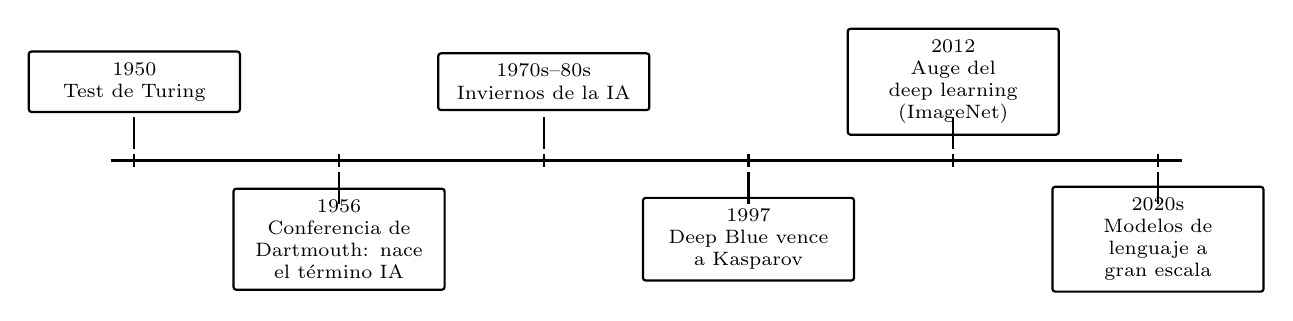
\begin{tikzpicture}[
  hito/.style={draw=black, thick, rectangle, rounded corners=1pt, inner sep=4pt, font=\scriptsize, text width=2.4cm, align=center}
]
\draw[thick] (-0.3,0) -- (13.3,0);
\foreach \x in {0,2.6,5.2,7.8,10.4,13} \draw[thick] (\x,0.08) -- (\x,-0.08);

\node[hito] at (0,1.0)    {1950\\Test de Turing};
\node[hito] at (2.6,-1.0) {1956\\Conferencia de Dartmouth: nace el término IA};
\node[hito] at (5.2,1.0)  {1970s--80s\\Inviernos de la IA};
\node[hito] at (7.8,-1.0) {1997\\Deep Blue vence a Kasparov};
\node[hito] at (10.4,1.0) {2012\\Auge del deep learning (ImageNet)};
\node[hito] at (13,-1.0)  {2020s\\Modelos de lenguaje a gran escala};

\draw[thick] (0,0.15)   -- (0,0.55);
\draw[thick] (2.6,-0.15) -- (2.6,-0.55);
\draw[thick] (5.2,0.15) -- (5.2,0.55);
\draw[thick] (7.8,-0.15) -- (7.8,-0.55);
\draw[thick] (10.4,0.15) -- (10.4,0.55);
\draw[thick] (13,-0.15) -- (13,-0.55);
\end{tikzpicture}
\caption{Línea de tiempo con algunos hitos de la historia de la IA.}
\end{figure}

\section{Agentes Inteligentes}
% Lectura: AIMA Cap. 2

\subsection{¿Qué es un Agente?}

\begin{definition}[Agente]
Un agente es cualquier entidad que \textbf{percibe} su ambiente mediante \textbf{sensores} y \textbf{actúa} sobre él mediante \textbf{actuadores}.
\end{definition}

La función del agente mapea percepciones a acciones: $f: P^* \rightarrow A$

\begin{figure}[H]
\centering
\begin{tikzpicture}[
  caja/.style={draw=black, thick, rectangle, rounded corners=1pt, minimum width=3cm, minimum height=1.4cm, font=\small}
]
\node[caja] (agente) at (0,0) {Agente};
\node[caja] (ambiente) at (6,0) {Ambiente};

\draw[-{Latex},thick] ([yshift=4mm]ambiente.west) -- node[above, font=\scriptsize]{Sensores (percepción)} ([yshift=4mm]agente.east);
\draw[-{Latex},thick] ([yshift=-4mm]agente.east) -- node[below, font=\scriptsize]{Actuadores (acción)} ([yshift=-4mm]ambiente.west);
\end{tikzpicture}
\caption{Ciclo agente-ambiente: el agente percibe el ambiente a través de sensores y actúa sobre él mediante
actuadores, en un ciclo continuo.}
\end{figure}

\begin{example}[PEAS de un taxi autónomo]
    La descripción PEAS de un taxi autónomo es:
    \begin{itemize}
        \item \textbf{Performance}: seguridad, tiempo de viaje, cumplir normas de tránsito, comodidad del pasajero.
        \item \textbf{Environment}: calles, otros vehículos, peatones, señales de tránsito, clima.
        \item \textbf{Actuators}: dirección, acelerador, freno, señales, bocina.
        \item \textbf{Sensors}: cámaras, GPS, velocímetro, sensores de proximidad (LIDAR/radar).
    \end{itemize}
\end{example}

\subsection{Racionalidad}

Un agente racional selecciona la acción que maximiza su \textbf{medida de desempeño} esperada, dado su conocimiento actual.

Depende de:
\begin{enumerate}
    \item La medida de desempeño
    \item El conocimiento previo del entorno
    \item Las acciones disponibles
    \item La secuencia de percepciones hasta el momento
\end{enumerate}

\subsection{Descripción PEAS}

Para caracterizar el ambiente de una tarea se usa PEAS:
\begin{itemize}
    \item \textbf{P}erformance (Medida de desempeño)
    \item \textbf{E}nvironment (Entorno)
    \item \textbf{A}ctuators (Actuadores)
    \item \textbf{S}ensors (Sensores)
\end{itemize}

\subsection{Naturaleza de los Ambientes}

\begin{tabular}{ll}
\toprule
\textbf{Dimensión} & \textbf{Valores posibles} \\
\midrule
Observabilidad & Completamente observable / Parcialmente observable \\
Agentes & Un solo agente / Multiagente \\
Determinismo & Determinista / Estocástico \\
Episodicidad & Episódico / Secuencial \\
Dinamismo & Estático / Dinámico \\
Tiempo & Discreto / Continuo \\
Conocimiento & Conocido / Desconocido \\
\bottomrule
\end{tabular}

\subsection{Tipos de Agentes}

\begin{enumerate}
    \item \textbf{Agente de reflejo simple}: actúa según la percepción actual (reglas condición-acción).
    \item \textbf{Agente de reflejo basado en modelos}: mantiene un estado interno del mundo.
    \item \textbf{Agente basado en objetivos}: considera metas para elegir acciones.
    \item \textbf{Agente basado en utilidad}: maximiza una función de utilidad.
    \item \textbf{Agente que aprende}: mejora su desempeño con la experiencia.
\end{enumerate}
